\section{Example: The Sleeping Barber}

Different concurrent programs produce different synchronisation problems.
Often these are presented in terms of colourful real-life scenarios.  One such
example is the sleeping barber.

A small barbershop is run by a single barber, and has several chairs.  When
there are no customers, the barber sleeps in his chair.  When a customer
arrives and finds the barber sleeping, he wakes up the barber, sits in the
chair, and sleeps while the barber cuts his hair.  If another customer arrives
in the meantime, he sleeps in one of the other chairs.  When the barber
finishes the haircut, he wakes up the customer, and holds the door open and
waits for him to leave.  If there are waiting customers, he wakes one up and
waits for him to sit in the chair; otherwise, he goes back to sleep.

%%%%%

\begin{slide}
\heading{The sleeping barber}

We will implement a monitor to solve this synchronization problem.  The
monitor will have the following methods:
%
\begin{description}
\item[getNextCustomer]
The barber wakes up a customer and waits for him to sit in the chair, or
sleeps until a customer arrives;

\item[getHaircut]
A customer arrives and waits until the barber is ready, then sits in the
chair;

\item[finishedCut]
The barber wakes up the customer, and waits for him to leave;

\item[waitForHaircut]
The customer waits for the barber to finish, then leaves.
\end{description}
%
Each pair of methods will involve a signal in each direction between the two
parties.
\end{slide}

\begin{slide}
\heading{Barber and customer processes}

The barber and customer processes must call the appropriate methods in order;
for example:
%
\begin{scala}
  def barber = thread("Barber"){
    while(true){
      sleep(Random.nextInt(500)); println("Barber ready")
      Barber.getNextCustomer; println("Barber cutting hair")
      sleep(Random.nextInt(500)+1000); println("Barber finished")
      Barber.finishedCut
  } }

  def customer(me: Int) = thread("Customer"+me){
    while(true){
      sleep(Random.nextInt(6000)); println("Customer "+me+" arrived")
      Barber.getHaircut; println("Customer "+me+" getting haircut")
      Barber.waitForHaircut; println("Customer "+me+" finished haircut")
  } }
\end{scala}
\end{slide}

%%%%%

\begin{slide}
\heading{Variables and conditions}

Each procedure will involve signalling to the other party.  We include a
condition for each signal.  However, in two cases it's possible that the
signal is sent before the other party is waiting for it; we use boolean
variables to cover these cases.

\begin{scala}
object Barber{
  /** Is the barber ready to cut hair, or finished the last cutting? */
  private var barberAvailable = false; private var barberDone = false

  private val lock = new Lock
  
  /** Conditions to signal that the barber is ready, the customer is ready,
    * the barber has finished cutting, and the customer has left. */
  private val barberAvailableC, chairOccupiedC, barberDoneC, customerLeftC =
    lock.newCondition
  ...
}
\end{scala}
\end{slide}

%%%%%

\begin{slide}
\heading{Sequence diagram}

\def\cx{4.0} \def\ba{8.5} \def\bd{11.5}
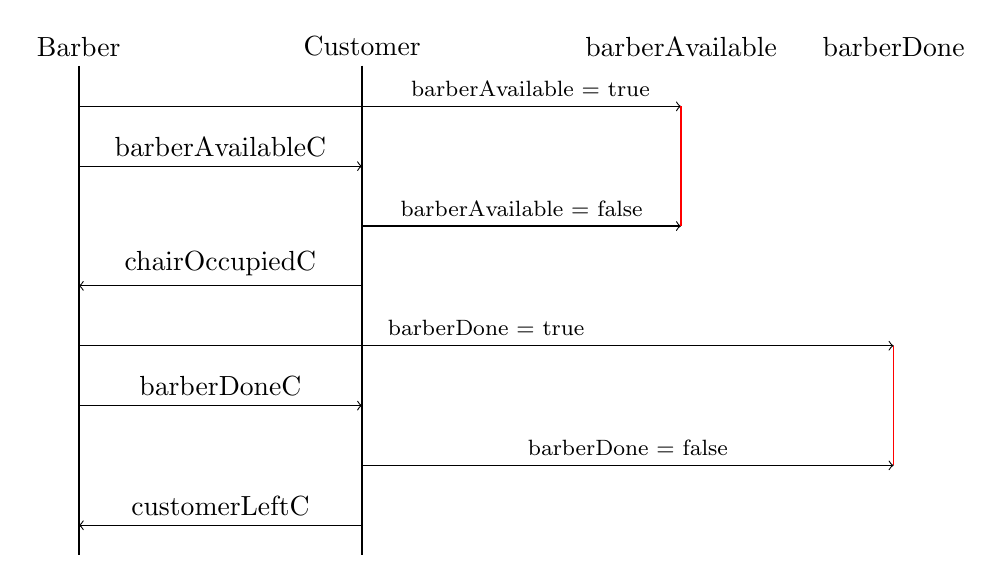
\begin{tikzpicture}[yscale = 0.76,xscale = 0.9]
\draw(0,0) node (b) {Barber};
\draw[black,thick] (b) -- ++ (0,-8.5);
\draw(\cx,0) node (c) {Customer};
\draw[black,thick] (c) -- ++ (0,-8.5);
\draw(\ba,0) node (ba) {\scalashape barberAvailable};
\draw(\bd,0) node (bd) {\scalashape barberDone};
%
\draw[->] (0,-1) -- 
  node[above,near end]{\footnotesize\scalashape barberAvailable = true}
  (\ba,-1);
\draw[->] (0,-2) -- node[above]{\scalashape barberAvailableC} (\cx,-2);
\draw[->] (\cx,-3) -- 
  node[above]{\footnotesize\scalashape barberAvailable = false}
  (\ba,-3);
\draw[red] (\ba,-1) -- (\ba,-3);
\draw[<-] (0,-4) -- node[above]{\scalashape chairOccupiedC} (\cx,-4);
%
\draw[->] (0,-5) -- node[above]{\footnotesize\scalashape barberDone = true}
   (\bd,-5);
\draw[->] (0,-6) -- node[above]{\scalashape barberDoneC} (\cx,-6);
\draw[->] (\cx,-7) -- node[above]{\footnotesize\scalashape barberDone = false}
   (\bd,-7);
\draw[red] (\bd,-5) -- (\bd,-7);
\draw[<-] (0,-8) -- node[above]{\scalashape customerLeftC} (\cx,-8);

\end{tikzpicture}
\end{slide}

%%%%%

\begin{slide}
\heading{The first two signals}

The barber signals that he is ready using |barberAvailableC|.  However, a
customer might not have arrived yet, so he also sets |barberAvailable|.  The
customer has to recheck |barberAvailable| when he awakes, in case another
customer has arrived and taken the slot. 

The barber then waits for a signal on |chairOccupiedC|.  There is only one
barber, and he must be waiting before the signal is sent, so nothing more is
needed. 
\end{slide}

%%%%%

\begin{slide}
\heading{The first two signals}

\begin{scala}
  /** Barber waits for next customer. */
  def getNextCustomer = lock.mutex{
    barberAvailable = true
    barberAvailableC.signal()                  // signal to a customer at (1)
    chairOccupiedC.await()                     // wait for signal (2)
  }

  /** Customer waits for barber to be available. */ 
  def getHaircut = lock.mutex{
    barberAvailableC.await(barberAvailable) // wait for barber (1)
    barberAvailable = false                   // clear for next round
    chairOccupiedC.signal()                   // signal to barber at (2)
  }
\end{scala}
\end{slide}

%%%%%

\begin{slide}
\heading{The third and fourth signals}

The barber signals he has finished on |barberDoneC|.  However, it's possible that
the customer isn't yet waiting, so he also sets |barberDone|.  No other
customer can be waiting on this signal, so nothing more is needed.

The barber then waits for a signal on |customerLeftC|.  Again he must be
waiting before the signal is sent, so nothing more is needed.
\begin{scala}
  def finishedCut = lock.mutex{
    barberDone = true; barberDoneC.signal()  // wake up customer at (3)
    customerLeftC.await()                        // wait for customer to leave (4)
  }

  def waitForHaircut = lock.mutex{
    if(!barberDone) barberDoneC.await()     // wait for barber to finish (3)
    assert(barberDone); barberDone = false  // clear for next round
    customerLeftC.signal()                     // signal to barber at (4)
  }
\end{scala}
\end{slide}




%%%%%
%%%%%%%%%%%%%%%%%%%%%%%%%%%%%%%%%%%%%%%%%%%%%%%%%%%%%%%
% \begin{slide}
% \heading{The status of the scenario}

% The scenario has four stages: the barber waiting for a customer; the customer
% sitting in the chair getting a haircut; the barber waiting for the customer to
% leave; the customer having left.   We therefore have a variable that records
% the current status:
% %
% \begin{scala}
% val barberAvailable = 0; 
% val chairOccupied = 1; 
% val doorOpen = 2; 
% val customerLeft = 3;
% var status = -1;
% \end{scala}
% \end{slide}

% %%%%%

% \begin{slide}
% \heading{The first two stages}

% The barber signals to a sleeping customer (if any), and waits until the chair
% is occupied.  The customer waits for the barber to be ready, occupies the
% chair, and signals to the barber.
% %
% \begin{scala}
% def GetNextCustomer = synchronized{
%   status = barberAvailable;
%   notify(); // wake up a sleeping customer
%   while(status!=chairOccupied) wait(); // wait for customer
% }

% def GetHaircut = synchronized{
%   while(status!=barberAvailable) wait(); // wait for barber
%   status = chairOccupied;
%   notifyAll(); // Signal to barber
% }
% \end{scala}
% \end{slide}

% %%%%%

% \begin{slide}
% \heading{The last two stages}

% The barber opens the door, signals to the customer, and waits for the customer
% to leave.  The customer waits for the barber to open the door, leaves, and
% signals to the barber.
% %
% \begin{scala}
% def FinishedCut = synchronized{
%   status = doorOpen;
%   notifyAll(); // signal to customer
%   while(status!=customerLeft) wait(); 
%     // wait for customer to leave
% }

% def WaitForHaircut = synchronized{
%   while(status!=doorOpen) wait(); // wait for barber to finish
%   status = customerLeft; 
%   notifyAll(); // Signal to barber
% }
% \end{scala}
% \end{slide}

% %%%%%

% \begin{selfnote}
% Note use of \SCALA{notifyAll()}

% Moral: identify the scenarios under which processes might be woken up; use
% state variables to ensure that processes wake up only under the appropriate
% circumstances, and only the appropriate number are woken up. 
% \end{selfnote}

%%%%%

\begin{slide}
\heading{Synchronisation problems}

Synchronisation problems like this can be difficult.  In order to come up with
a correct and understandable design, it is useful to use state variables that
indicate which processes are in different states, at least in \emph{quiescent
  states} when no processes
are running or runnable.

For example, the |barberAvailable| variable records (in quiescent states) that
the barber is waiting for a signal in |getNextCustomer|.  The customer that
will be served next clears this variable before signalling to the barber and
releasing the lock.

The |barberDone| variable records (in quiescent states) that the barber is
waiting for a signal in |finishedCut|.  The current customer clears this
variable before signalling to the barber and releasing the lock.
\end{slide}

%%%%%

% {\advance\slideheight by 3mm
% \begin{slide}
% \heading{Synchronisation problems}

% For example, with the sleeping barber, when no processes are running or
% runnable:
% %
% \begin{itemize}
% \item
% If \SCALA{barberAvailable = true} then the barber is waiting in
% \SCALA{GetNextCustomer} and no customers are in the module;

% \item
% If \SCALA{status == chairOccupied} then the barber is not in the module, one
% customer might be waiting in \SCALA{WaitForHaircut} (or has finished
% \SCALA{GetHairCut} and not yet started \SCALA{WaitForHairCut}), and other
% customers might be waiting in \SCALA{GetHairCut}.
% \end{itemize}
% %
% And
% %
% \begin{itemize}
% \item
% If \SCALA{status == doorOpen} then the barber is waiting in
% \SCALA{FinishedCut}, one customer is running or runnable in
% \SCALA{WaitForHairCut}, and other customers might be waiting in
% \SCALA{GetHairCut};

% \item
% If \SCALA{status == customerLeft} then the barber is running or runnable in
% \SCALA{FinishedCut}, or has exited \SCALA{FinishedCut}.
% \end{itemize}
% \end{slide}}

%%%%%

\begin{slide}
\heading{Synchronisation problems}

In other synchronisation problems, it can be useful to keep track of:
%
\begin{itemize}
\item 
How many processes are waiting in various waits;

\item
How many processes have completed operations (or maybe the difference between
the number of times two matching operations have been completed).
\end{itemize}

To track down bugs, it can be useful to:
\begin{itemize}
\item write lots of assertions;

\item use logging, particularly of the sending and receiving of
signals.
\end{itemize}
\end{slide}
